\subsection{Descent: the case of coverings}

Let X, Y be topological spaces and let \(f: X \to Y\) be a surjective continuous map. Let \((Z, p)\) be a covering of X and let \(\tau\) be a descent datum relative to f on Z.

If \(f\) is proper and separated (resp. if \(f\) is open), the descent datum \(\tau\) is effective and the Y-space \(Z/R_{\tau}\) is an étale space (IV, p.~389, prop. 5). It is even a covering of Y if \(f\) has a continuous section in a neighborhood of each point (I, p.~72, prop. 3) or if Z is a locally finite covering of X (I, p.~77, cor. 4). This section is devoted to highlighting other conditions under which \(Z/R_{\tau}\) is a covering of Y.

Let us first prove a lemma.

Lemma 1. --- Let B, B' be topological spaces and let \(f: \mathrm{B}' \to \mathrm{B}\) be a continuous map. If the fibered square \(\mathrm{B}' \times_{\mathrm{B}} \mathrm{B}'\) is locally connected, then the topological space \(\mathrm{B}'\) is locally connected.

Let \(a\) be a point of \(\mathrm{B}'\) and let V be a neighborhood of \(a\) . Suppose that the fibered square \(\mathrm{B}' \times_{\mathrm{B}} \mathrm{B}'\) is locally connected, and let W be a connected neighborhood of \((a, a)\) in \(\mathrm{B}' \times_{\mathrm{B}} \mathrm{B}'\) which is contained in \(\mathrm{V} \times \mathrm{V}\) . Set \(\mathrm{U} = \mathrm{pr}_1(\mathrm{W})\) . The set U is contained in V, and is connected since the image of a connected set under a continuous map is connected. If \(\Delta_{\mathrm{B}'}\) denotes the diagonal of \(\mathrm{B}' \times_{\mathrm{B}} \mathrm{B}'\) , the map \(\mathrm{pr}_1 \mid \Delta_{\mathrm{B}'}: \Delta_{\mathrm{B}'} \to \mathrm{B}'\) is a homeomorphism. Since U contains \(\mathrm{pr}_1(\mathrm{W} \cap \Delta_{\mathrm{B}'})\) and \(\mathrm{W} \cap \Delta_{\mathrm{B}'}\) is a neighborhood of \((a, a)\) in \(\Delta_{\mathrm{B}'}\) , U is a neighborhood of \(a\) in \(\mathrm{B}'\) . This proves the lemma.

PROPOSITION 6. --- Let

\pandocbounded{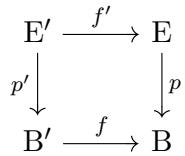
\includegraphics[keepaspectratio]{images/part003_c1a9b5e7.jpg}}

a Cartesian square. We assume that the map f is proper, separated, and surjective, and we make one of the following hypotheses:

\begin{enumerate}
\def\labelenumi{(\roman{enumi})}
\item
  The fibers of f are locally connected and the fibered square \(B^{\prime} \times_{B} B^{\prime}\) is locally connected.
\item
  The fibers of \(f\) are finite, the diagonal \(\Delta_{\mathrm{B}^{\prime}}\) of \(\mathrm{B}^{\prime}\times_{\mathrm{B}}\mathrm{B}^{\prime}\) is open in \(\mathrm{B}^{\prime}\times_{\mathrm{B}}\mathrm{B}^{\prime}\) and \(\mathrm{B}^{\prime}\times_{\mathrm{B}}\mathrm{B}^{\prime} - \Delta_{\mathrm{B}^{\prime}}\) is a locally connected space.
\end{enumerate}

Then, if \((\mathrm{E}^{\prime}, p^{\prime})\) is a covering, \((\mathrm{E}, p)\) is a covering.

Since the map \(f\) is universally strict (I, p.~20, corollary), the map \(p\) is étale (I, p.~31, prop. 8) and separated (I, p.~27, prop. 4). We shall assume, as is permissible, that \(\mathrm{E}' = \mathrm{B}' \times_{\mathrm{B}} \mathrm{E}\) .

Let \(a\) be a point of B; the aim is to show that the point \(a\) has a neighborhood W such that the W-space \((\mathrm{E_W}, p_{\mathrm{W}})\) is a trivializable covering. Set \(\mathrm{B}_a^\prime = f^{-1}(a)\) and set \(\mathrm{E}_a^\prime = (p')^{-1}(\mathrm{E}_a)\) . The map \(t_a: \mathrm{E}_a^\prime \to \mathrm{B}_a^\prime \times \mathrm{E}_a\) defined by \(t_a(y) = (p'(y), f'(y))\) is a \(\mathrm{B}_a^\prime\) -isomorphism (I, p.~9, prop. 4), hence \(\mathrm{E}_a^\prime\) is a trivializable covering of \(\mathrm{B}_a^\prime\) and \(t_a\) is a trivialization of this covering.

Let us prove that there exists a neighborhood \(V'\) of \(B'_{a}\) in \(B'\) and a continuous trivialization t of the covering ( \(E_{V'}', p_{V'}\) ) that extends \(t_{a}\) . Under hypothesis (ii), \(B'_{a}\) is finite and its points possess pairwise disjoint open neighborhoods over which the covering \(E'\) is trivializable, whence the assertion in this case. Under hypothesis (i), \(B'_{a}\) is locally connected, as is B' (IV, p.~390, lemma 1); since the map f is proper and separated, \(B'_{a}\) is compact and two distinct points have disjoint neighborhoods in B', so that the pair (B', \(B'_{a}\)) satisfies property (PCV) (I, p.~37, lemma 1). The assertion therefore follows from cor. 2 of I, p.~90.

Since \(f\) is proper, there exists a neighborhood \(V\) of \(a\) in \(B\) such that \(V'\) contains \(f^{-1}(V)\) (lemma, I, p.~75). One may thus assume that \(V' = f^{-1}(V)\) .

Equip the \(V'\)-spaces \(V' \times E_{a}\) and \(E_{V'}' = V' \times_{B} E\) with their canonical descent data relative to \(f_{V}: V' \to V\) . We shall show that, after possibly shrinking V and \(V'\), the isomorphism of \(V'\)-spaces \(t: E_{V'}' \to V' \times E_{a}\) that we have just defined is compatible with the descent data, that is, we have \(t(b_{1}', x) = t(b_{2}', x)\) if \((b_{1}', b_{2}') \in V' \times_{V} V'\) and \(x \in E_{f(b_{1}')}\) . Denote by \(\widetilde{t}\) the map \(pr_{2} \circ t: E_{V'}' \to E_{a}\) .

Let us set \(V'' = V' \times_{V} V'\) ; consider it as a \(V'\)-space by means of the first projection. The map \(((b_{1}', b_{2}'), x) \mapsto ((b_{1}', b_{2}'), (b_{1}', x))\) from \(V'' \times_{V} E\) into \(V'' \times_{V'} E'\) is an isomorphism of \(V''\)-spaces; this shows that \(V'' \times_{V} E\) is a covering of \(V''\) .

For \(i=1,2\) , we define a map \(u_{i}\colon V^{\prime\prime}\times_{V}E\to V^{\prime\prime}\times E_{a}\) by setting \(u_{i}(b_{1}^{\prime},b_{2}^{\prime},x)=(b_{1}^{\prime},b_{2}^{\prime},\widetilde{t}(b_{i}^{\prime},x))\) ; these are trivializations of the covering \(V^{\prime\prime}\times_{V}E\) . Let \(W^{\prime\prime}\) be the set of points \(w\in V^{\prime\prime}\) over which these trivializations \(u_{1}\) and \(u_{2}\) coincide; it contains \(B_{a}^{\prime}\times B_{a}^{\prime}\) , as well as the diagonal \(\Delta_{V'}\) . Let us prove that \(W^{\prime\prime}\) is a neighborhood of \(B_{a}^{\prime}\times B_{a}^{\prime}\) . Under hypothesis (i), this follows from cor. 2 of I, p.~80, since \(B^{\prime}\times B^{\prime}\) is locally connected. Under hypothesis (ii), \(W^{\prime\prime}\) contains a neighborhood of \((B_{a}^{\prime}\times B_{a}^{\prime})-\Delta_{B_{a}^{\prime}}\) in \((B^{\prime}\times_{B}B^{\prime})-\Delta_{B^{\prime}}\) , since this set is locally connected (loc. cit.). Since \(\Delta_{V'}\) is open in \(B^{\prime}\times_{B}B^{\prime}\) , \(W^{\prime\prime}\) is a neighborhood of \(B_{a}^{\prime}\times B_{a}^{\prime}\) in \(V^{\prime\prime}\) .

Since \(f\) is proper, the canonical map \(f''\) of \(\mathrm{B}' \times_{\mathrm{B}} \mathrm{B}'\) into B is proper, because it is the composite of the projection \(\mathrm{pr}_{1} \colon \mathrm{B}' \times_{\mathrm{B}} \mathrm{B}' \to \mathrm{B}'\) and of the mapping \(f\) .

By the lemma of I, p.~75, there exists a neighborhood W of a in V such that \((f'')^{-1}(\mathrm{W})\) is contained in \(W''\); set \(W'=(f')^{-1}(\mathrm{W})\), which is a subset of \(V'\) and the isomorphism of étale spaces \(t: E_{W'}' \to W' \times E_a\) is compatible with the canonical descent data relative to the map \(f_W: W' \to W\) . It follows from the corollary (IV, p.~388) that the

W-étale spaces \(E_{W}\) and \(W \times E_{a}\) are isomorphic. In particular, \(E_{W}\) is a trivializable covering, whence the proposition.

COROLLARY 1. --- Let E and B be topological spaces, \(p\colon\mathrm{E}\to\mathrm{B}\) a continuous map and \((\mathrm{A}_{i})_{i\in\mathrm{I}}\) a locally finite closed covering of B such that for every pair \((i,j)\in\mathrm{I}\times\mathrm{I}, i\neq j\) , the intersection \(\mathrm{A}_{i}\cap\mathrm{A}_{j}\) is a locally connected space. Then, for the B-space \((\mathrm{E},p)\) to be a covering, it is necessary and sufficient that, for every \(i\in\mathrm{I}\) , the \(\mathrm{A}_{i} \)-space \((p^{-1}(\mathrm{A}_{i}),p_{\mathrm{A}_{i}})\) be a covering of \(\mathrm{A}_{i}\) .

The condition is necessary (cf. I, p.~69). Conversely, let B' denote the topological sum space of the family \((\mathrm{A}_{i})_{i\in\mathrm{I}}\) and \(f\colon B'\to B\) the canonical map. The map f is closed (TG, I, p.~6, prop. 4), separated (I, p.~27, remark 5), with finite fibers, hence proper (TG, I, p.~75, th. 1); it is also surjective. The diagonal \(\Delta_{B'}\) , being equal to \(\bigcup_{i\in I}A_{i}\times_{B}A_{i}\) , is open in \(B'\times_{B}B'\) . Finally, the space \((\mathrm{B}'\times_{\mathrm{B}}\mathrm{B}')-\Delta_{\mathrm{B'}}\) is homeomorphic to the sum space of the family \((\mathrm{A}_{i}\cap\mathrm{A}_{j})\) , \((i,j)\in\mathrm{I}\times\mathrm{I}\) , \(i\neq j\) ; it is therefore locally connected. Hypothesis (ii) of proposition 6 is satisfied. If for every i, \(p^{-1}(\mathrm{A}_{i})\) is a covering of \(A_{i}\) , \(E'\) is then a covering of \(B'\) , hence E is a covering of B.

COROLLARY 2. --- Let X and Y be topological spaces and let \(f\colon X \to Y\) be a proper, separated, and surjective map. Moreover, assume one of the following hypotheses:

\begin{enumerate}
\def\labelenumi{(\roman{enumi})}
\item
  The fibers of f, as well as the space \(X\times_Y X\), are locally connected;
\item
  The fibers of \(f\) are finite, the diagonal \(\Delta_{\mathrm{X}}\) of \(\mathrm{X} \times_{\mathrm{Y}} \mathrm{X}\) is open in \(\mathrm{X} \times_{\mathrm{Y}} \mathrm{X}\) and the space \((\mathrm{X} \times_{\mathrm{Y}} \mathrm{X}) - \Delta_{\mathrm{X}}\) is locally connected. Then, every descent datum relative to \(f\) on a covering of \(\mathrm{X}\) is effective, and the quotient space is a covering of \(\mathrm{Y}\) .
\end{enumerate}

Let Z be a covering of X and let \(\tau\) be a descent datum relative to f on Z. By proposition 5 (IV, p.~389), the descent datum \(\tau\) is effective, in other words the square

\pandocbounded{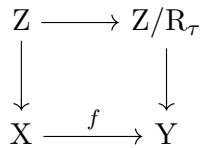
\includegraphics[keepaspectratio]{images/part003_fd3d7e4d.jpg}}

is a Cartesian square. The hypotheses of proposition 6 (IV, p.~391) are then satisfied. Consequently, \(Z/R_{\tau}\) is a covering of Y.

PROPOSITION 7. --- Let X and Y be topological spaces and let \(f: X \to Y\) be a continuous and surjective map. Suppose that Y is deloopable and that the map f is open and has the path-lifting property. Then, every descent datum relative to f on a covering of X is effective, and the quotient space is a covering of Y.

Let \((Z,p)\) be a covering of X and let \(\tau\) be a descent datum relative to f on Z. Since the map f is surjective and open, it follows from prop. 5 of IV, p.~389, that the descent datum \(\tau\) is effective. Let \(T = Y/R_{\tau}\) denote the quotient Y-space; its projection q is étale (loc. cit.), and it is also separated (I, p.~27, prop. 4).

By hypothesis, the map f has the path lifting property, as does the map p, since Z is a covering of X (III, p.~302, corollary 2 of prop. 3). Consequently, the same holds for the map \(p \circ f\) , hence for the map q. Therefore (cf.~IV, p.~341, remark 2), T is a covering of Y. The proposition is thus proved.

Remark. --- Let X and Y be topological spaces and let \(f: X \rightarrow Y\) be a map. For every descent datum relative to f on a covering of X to be effective, and for the quotient space to be a covering of Y, it is necessary that f be strict and that \(f(X)\) be an open and closed subset of X.

Indeed, identify the X-space X with \(X \times_{Y} Y\) and endow it with its canonical descent datum relative to f. The quotient space is identified with \(f(\mathrm{X})\) , equipped with the quotient topology of the topology of X for the equivalence relation defined by f. If this is a covering of Y, the space \(f(\mathrm{X})\) is then identified with an open and closed subset of Y and the map f is strict.

